\Chapter{Saját tűz implementációk}

% TODO: Ide kellene sorban bemutatni az implementációkat!

\section{Fejlesztői környezet}

\subsection{OpenGL}

% NOTE: Az OpenGL alapvetően egy nyílt grafikus függvénykönyvtár (library).

Az OpenGL egy platform- és nyelvfüggetlen, nyílt grafikus függvénykönyvtár (\textit{library}) 2 és 3D-s vektorgrafikus megjelenítéshez. Az API használatán keresztül elérhetjük a grafikus kártyát, így hardveresen gyorsított megjelenítést valósíthatunk meg a számítógépen. A Silicon Graphics Inc. kezdte fejleszteni, majd 1992-ben adták ki először. Széles körben alkalmazzák az iparban, többek között számítógéppel segített tervezésben (CAD), virtuális valóságokban, tudományos vizualizációk során, információ szemléltetésben, repülő szimulátorokban és végül, de nem utolsó sorban a számítógépes játékokban. 2006 óta a nonprofit Khronos csoport vette át a fejlesztését \cite{wikiOGL}.

\subsection{Freeglut}

Az OpenGL Utility Toolkit (GLUT) egy olyan platformfüggetlen könyvtár, amely gondoskodik a rendszerspecifikus feladatokról, melyekre ablak kezelés, OpenGL kontextusok inícializálása és bemeneti események (billentyűzet, egér) kezelése esetén van szükség. Használata gyorsan elterjedt, ugyanis egyszerű, széles körben elérhető és hordozható volt. Azonban 1998 augusztusa óta nem fejlesztették tovább, így a kód elöregedett. A FreeGLUT egy ingyenes, nyílt forráskódú alternatíva ehhez. Továbbra is fejlesztés alatt áll, és a GLUT-hoz képest több funkcióval, és kevesebb hibával rendelkezik \cite{freeGlut}.

\subsection{OpenGL Extension Wrangler Library (GLEW)}

A GLEW egy platformfüggetlen C/C++ könyvtár, amely segíti az OpenGL bővítmények (\textit{extensions}) lekérdezését és betöltését. Futásidőben megállapítja, hogy az adott célhardveren mely OpenGL bővítmények támogatottak. Az összes bővítményt kigyűjti egyetlen, a számítógép által generált header fájlba, mely a hivatalos bővítmény listából készül. Több operációs rendszeren is tesztelték, többek között Windows-on, Linux-on, Mac OS X-en, FreeBSD-n, Irix-en és Solaris-on. A 2.1.0 verzió már az OpenGL 4.6-os verzióját is támogatja \cite{glew}.

\subsection{OpenGL Mathematics}

Az OpenGL Mathematics (GLM) egy OpenGL Shading Language (GLSL) specifikációkon alapuló, csak header fájlokból álló C++ könyvtár a grafikus szoftverekhez. Olyan osztályokkal és függvényekkel szolgál, melyek elnevezési konvenciói és funkciói megegyeznek a GLSL-ben találhatókkal, íg aki a GLSL-t ismeri, az tudja használni a GLM-et is. Ezen felül azonban olyan bővítmény rendszerrel is bír, mely szintén megfelel a GLSL bővítmény konvencióknak, és ez további képességekkel szolgál: mátrix transzformációk, random számok, zaj, stb \cite{glm}.

\subsection{Simple OpenGL Image Library}

A Simple OpenGL Image Library (SOIL) egy platformfüggetlen C könyvtár, melyet elsősorban textúrák betöltésére használhatunk. Elvégzi a szükséges lépéseket, melyeket az OpenGL igényel textúrák előkészítésénél. A könyvtár segítségével nem csak betölteni, hanem menteni is lehet képeket. Mivel kis méretű, első sorban statikus könyvtárként való használatra szánták. Tesztelték Windows-on, Linux-on és Mac-en \cite{soil}.

\section{A kiinduló projekt}

% domborzat
Az következő implementációkat egy már elkészült, korábbi projekt keretein belül jelenítem meg. GLEW 2.0-t használtam, tehát az OpenGL 4.5-ös verziójának funkciói álltak rendelkezésemre. 

A projekt egy általam készített domborzatot tölt be, melyhez az adatokat különböző képfájlokból olvassa be. A magasságértékeket egy szürkeárnyalatos kép képpontjaiban tároltam, a hozzájuk tartozó nedvesség értékeket pedig egy másik, szintén szürkeárnyalatos képfájlban. A színeket egy olyan képből olvastam ki, ahol az egyik tengely a magasságot, a másik pedig a nedvességet jelölte, így az adott csúcspont színe a magasság és nedvesség értékéből kapható meg. A domborzathoz 260100 darab csúcspontot használtam fel. Az égbolt és a hold is gömb alakú, melyekhez a csúcspontokat, textúra koordinátákat, normál vektorokat és az ezekhez szükséges indexeket is az általam készített Sphere osztály generálja. Az ég 4225, a hold 1089 csócspontból áll. Mindezek megjelnítéséért és aktualizálásáért az \texttt{Environment} osztály felel.

A program így 400 és 450 fps (frame per secundum) között fut, azaz másodpercenként nagyjából ennyiszer rajzolja ki a színteret.

\subsection{Textúrák}

A textúrák betöltéséért, paraméterezéséért, illetve az egyéb információkkal szolgáló képek beolvasásáért a TextureLoader osztályom felel a SOIL könyvtár segítségével. 

% TODO: Egy SOIL hivatkozás is kellhet ide még.

Textúrát betölthetünk egyszerűen a \texttt{SOIL\_load\_OGL\_texture} függvényével is , ebben az estben csupán a textúra paramétereket kell beállítani, azaz hogy a kép nyújtása vagy zsugorítása esetén milyen módszerrel mintavételezze a textúrát, illetve a $[0, 1]$ intervallumot meghaladó textúra koordináták esetén milyen módszerrel töltse ki az érintett részeket. Ennek a hátránya azonban, hogy a mintavételezési lehetőségek között nincs olyan, amely a zsugorított textúrák esetén szép képet eredményezne. Ezért készítettem a \texttt{loadMipMappedTexture} függvényt, amely mipmap-et is generál a betöltött képhez a \texttt{glGenerateMipmap} függvény segítségével. Mivel itt csak a \texttt{SOIL\_load\_image} függvényt használom a kép beolvasásához, a textúra betöltéséről, azonosító generálásról és a pixel tárolási módról is gondoskodni kellett. Előnye viszont, hogy az adott kép több, kisebb méretben is legenerálódik, így a zsugorított textúrák is sokkal szebben mutatnak.

A \texttt{loadImage} függvény segítségével lehet egyszerűen képeket beolvasni. Ehhez társul a \texttt{getPixelColor} függvény is, mely visszaadja a koordinátái segítségével megadott pixel RGB színét. Az értékeket a $[0, 1]$ intervallumra képeztem le ($\frac{\text{pixel érték}}{255}$).

\subsection{Shader-ek}

Az OpenGL renderelési pipeline-jának egyes részei a programozó által írt shader programok segítségével befolyásolható. A ``modern'' OpenGL-ben többféle shader is használható. Ezek közül a legalapvetőbbek a vertex és fragment shader-ek. A shadereknek vannak különféle be- és kimenetei, melyeket a programozó adhat meg. A feldolgozásuk is a programozóra van bízva, de a pipeline működéséhez néhány előre definiált változónak is értéket kell adni (pl.: \texttt{gl\_Position}). A vertex shader dolgozza fel a bemenetként kapott pontokat (vertex), tehát nagyjából annyiszor fut le, ahány pontot kirajzolunk. A kimenetként minimum produkálnia kell egy pontot, emellett pedig egyéb, a programozó által definiált információkat is továbbadhat a többi shader-nek. A fragment shader képpontonként fut le, ugyanis a bemenetei segítségével ez állítja elő a képpont végső színét.

A shader-ek betöltésére és használatára egy külső könyvtárat használtam, melynek funkciói a \texttt{tdogl} névteren belül találhatóak. Ez elvégzi a szükséges OpenGL beállításokat, és nagyban leegyszerűsíti az árnyaló programok használatát. A shader-ek Phong-féle megvilágítási modellt valósítják meg. A szebb eredmény érdekében a számításokat képpontonként végzik, azaz a modellt a fragment shader-ben implementáltam. Ezen belül is kétféle változatot készítettem. Az egyikben csúcspontonként megadhatók különböző színek, ezt használtam a domborzat kirajzolásához. A másikban pedig egy objektum kirajzolásához egy szín adható meg uniform-ként, tehát így minden csúcspont színe egyforma. Utóbbit azon objektumokra alkalmaztam, melyek színét leginkább a textúra definiálja (az égbolt és a hold).

\subsection{Camera osztály}

% camera: transzformációk, ütközésvizsgálat, időmérés
A nézeti és projekciós mátrixok transzformációit a Camera osztályban tartom számon. Ez az osztály felel a térben való mozgásért, illetve az $Y$ (jobbra/balra fordulás) és az $X$ (fel/le nézés) tengely mentén való forgatásért. 
Az elfordulási szögek radiánban vannak számontartva, és a túlcsordulások elkerülése érdekében az $Y$ tengely menti fordulást a $[-\pi \cdot 2, \pi \cdot 2]$, az X tengely mentit pedig $\left[-\frac{\pi}{2}, \frac{\pi}{2}\right]$ intervallumra szűkítem le. Nem tartom számon külön a nézeti, és külön a projekciós mátrixot, hanem a kettő szorzatából eredő \texttt{camera} mátrixot használom. Az \texttt{updateCamera} metódust minden kirajzolás elején meg kell hívni, ugyanis ez számolja ki a pillanatnyi camera mátrixot, és állítja be minden shader-ben uniform-ként. 

Egyszerű ütközésvizsgálatra is ebben az osztályban van lehetőség, ehhez meg kell adni az akadályok pozícióinak listáját, illetve egy akadály sugarát, melyet az alapjának a befoglaló köre határoz meg. Az ütközésvizsgálat csak kétdimenziós, az $XZ$ síkon történik. Eredetileg fákkal történő ütközésvizsgálathoz lett írva, de a tűzön való áthaladást is könnyedén meg lehet vele akadályozni, ha szükséges. A kamera új pozíciójának kiszámítása előtt letárolom a pillanatnyi pozíciót, és amennyiben az új pozícióban ütközés történik, az előző pozíció értéke marad meg. Az ütközést rendkívül egyszerűen állapítom meg: a kamera $(X, Z)$ pozíciója és az akadály $(X, Z)$ pozíciója közti távolságot számolom ki minden akadályra. Amennyiben ez a távolság kisebb, mint a megadott sugár, ütközés történt. Nem golyóálló a módszer, viszont rendkívül gyors.

Az új pozíció meghatározásához számon kell tartani az előző kirajzolás óta eltelt időt, hiszen ha minden kirajzolás esetén ugyanannyival mozdulna el a kamera az adott irányba, akkor a hardver gyorsaságától is függne a sebessége. Mivel a \texttt{glutGet(GLUT\_ELAPSED\_TIME)} felbontása nem túl nagy a mai hardverek sebességéhez képest, előfordulhat, hogy többször is nullát kapunk az eltelt idő számításakor, így a kamera nem mozdul. Helyette a Windows \texttt{QueryPerformanceCounter} függvényét használtam, mely megbízhatóbb e téren.

\subsection{Frame per secundum mérés}

% fps mérő
Annak érdekében, hogy a kirajzolt jelenetek számításigényéről információt szerezzünk a későbbiekben, szükséges volt egy fps mérő implementálása is. Ezt két függvény segítségével valósítottam meg: \texttt{calcFps} és \texttt{printFps}. Előbbi kirajzolásonként kiszámítja az aktuális fps-t, amelyet az $\frac{1}{\text{eltelt idő (sec)}}$ képletből számoltam. Utóbbi a refreshTime változóban (ms) meghatározott időközönként kiírja az arra az intervallumra vonatkoztatott átlag fps-t, amelyet az fps-ek összege és a kirajzolt képek számának a hányadosa ad meg. A képernyőre való kiíratáshoz a \texttt{glutBitmapCharacter} függvényt használtam, amely bitmap karaktereket ír ki a képernyőre. 

\section{Kétdimenziós sprite, illetve billboard tűz}

\subsection{SpriteFire osztály}

% sprite konstruktor
A két kétdimenziós megvalósítások közül a sprite változat az alapvetőbb, így azzal kezdtem az implementációt. A \texttt{SpriteFire} osztály konstruktorának meg kell adni a tűz árnyalására készített shader program és a camera objektum pointerét, illetve a pozíciót, ahol szeretnénk megjeleníteni. Opcionális paraméterként megadható, hogy szeretnénk-e a 90 fokkal elfordítva is kirajzolni, illetve a mérték (scale/skála), amellyel nagyítani vagy kicsinyíteni szeretnénk a tüzet. Mivel az objektum magassága alapártelmezetten 1 lesz, utóbbi paraméterrel tulajdonképpen egyben a magasságát is megadjuk. A konstruktor letárolja ezen paramétereket, majd beállítja a modell transzformációs mátrixot (az egységmátrixot eltolja a pozíció vektorral) és a csúcspontok számát, végül meghívja a \texttt{loadVAO} metódust.

% LoadVAO()
Az internetről egy olyan textúrát töltöttem le, melyen egy tűz minden állapota egy képen szerepel. Összesen 32 jelenetből áll majd az animáció, így egészen folyékony hatást kelt. Ezt a loadVAO metódus a \texttt{TextureLoader} osztály \texttt{loadMipMappedTexture} metódusa segítségével tölti be. 

% Vertex Array Object
A \texttt{loadVAO} metódus elkészíti a vertex array object-et (VAO). A VAO egy olyan objektum az OpenGL-ben, amely eltárolja a pontok adatait, és a pontok kirajzolásához szükséges infromációkat. A pontok Vertex Buffer Object-ekben (VBO) vannak tárolva, egy VAO-hoz több VBO is tartozhat.

\begin{wrapfigure}{r}{0.25\textwidth}
 \centering
 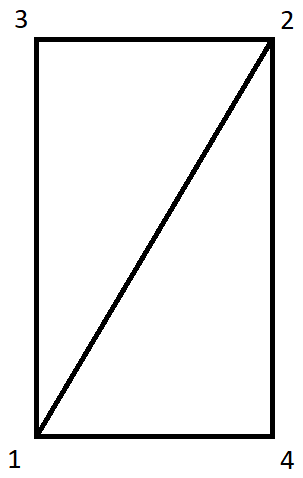
\includegraphics[width=0.25\textwidth]{kepek/billboardFrame.png}
 \caption{A billboard váza a csúcspontokkal.}
 \label{fig:spriteFrame}
\end{wrapfigure}

Minden VBO-hoz meg kell határozni, hogy az abban tárolt adatokat a shader program melyik attribútumán keresztül kapja meg. Mivel ezek az attribútumok alapértelmezetten le vannak tiltva, először külön engedélyezni kell őket. 

%calculateSpriteVertices()
A pontok meghatározását a \texttt{calculateSpriteVertices} metódus végzi. A textúrán 4 sorban és 8 oszlopban helyezkednek el rajta az állapotok, tehát egy állapot oldalainak aránya 2:1. Ez azt jelenti hogy a megjelenítésnél egy téglalapra kell ráhúzni képeket. A téglalapot természetesen 2 háromszög alkotja, amint az az \ref{fig:spriteFrame}. ábrán is látszik. 
Mivel az alakzatot az $Y$ tengely körül kell majd a későbbiekben forgatni, érdemes úgy definiálni a pontokat, hogy a téglalap alsó élének középpontja az origóba essen, hogy az a forgatás során egy helyben maradjon. A téglalap síkja pedig az $XY$ síkkal esik majd egybe, mert így egyszerűbb definiálni. Konkrét koordinátákkal is meghatározhatnám a téglalapot, de akkor minden kirajzolás esetén a modellmátrixot a skála paraméternek megfelelően skálázni kell. Hogy ezt a műveletet megspóroljam, eleve a skála segítségével határozom meg a koordinátákat. Az $Y$ koordináták a 0 vagy a skála értékét veszik fel, az $X$ koordináták azonban a $\pm \frac{\text{skála paraméter}}{4}$ értékeket, hiszen a magasság felét még az origó is kettéosztja. A pontokat az óramutató járásának irányával ellentétes sorrendben érdemes megadni, hogy a későbbiekben szükség esetén könnyen lehessen belőlük normálvektort számítani. Így tehát az első háromszög pontjai az 1, 2, 3 pontok, a másodikéi pedig 1, 4, 2. A pontokat ebben a sorrendben kell tárolni, ehhez mindig a C++ standard könyvtárának vektor típusú tárolóját használom, ugyanis kezelése könnyű, dinamikus a mérete és felszabadítja a lefoglalt helyet maga után.

%calculateNextTextureCoordinates()
Az ezekhez a pontokhoz tartozó textúra koordinátákat a \texttt{calculateNextTextureCoordinates} metódussal állítom elő. Mivel egy képen van több állapotom, ezek az értékek állapotról állapotra változnak. Egy adattag (\texttt{m\_iActualFrame}) segítségével számon tartom, hogy éppen hanyadik állapotnál járok, és ebből a számból határozom meg a hozzá tartozó koordinátákat. A számozást 0-tól kezdem. Először a sor és oszlopszámot kell kiszámolni hozzá. A sort az $\frac{\text{állapot sorszáma}}{\text{oszlopok száma}}$ hányados egész része adja meg, az oszlopot pedig az előbbi osztás maradéka (modulo művelet). A textúra koordináták a bal felső sarokból $(0, 0)$ indulnak, és a jobb alsó sarok $(1, 1)$ felé nőnek. Az adattagok között számon tartom, hogy egy állapot a textúra koordináta-rendszernek megfelelően milyen széles (\texttt{m\_fColumnstep}), és milyen magas (m\_fRowstep). Ennek megfelelően például az állapot bal felső pontjának $(u, v)$ koordinátája az 
\begin{align*}
u &= \text{adott oszlop} \cdot \text{szélesség}, \\
v &= \text{adott sor} \cdot \text{magasság}, 
\end{align*}
a jobb alsó pedig az  
\begin{align*}
u &= (\text{adott oszlop} + 1) \cdot \text{szélesség}, \\
v &= (\text{adott sor} + 1) \cdot \text{magasság} 
\end{align*}
egyenletek alapján kapható meg. Az így kapott $(u, v)$ koordinátákat a téglalap objektum pontjainak megfelelő sorrendben kell megadni, azaz 1, 2, 3, 1, 4, 2, ahol például 1 a bal alsó, 2 a jobb felső ponthoz tartozó koordináták. A metódus utolsó lépéseként növeljük az állapot sorszámát tároló adatag értékét eggyel, ügyelve arra, hogy az utolsó állapotot követően nullázzuk.

%VAO generálás
Ezek után generálunk egy VAO-t és a két vektort, melyeket az előbbi funkciókkal állítottunk elő, külön-külön VBO-k segítségével tároljuk a VAO-ban. A két VBO között fontos különbség, hogy amíg a pontokat statikus objektumként tároljuk le, addig a textúra koordinátákat dinamikusként kell, ugyanis ennek a VBO-nak a tartalma fog változni az animáció során. Ezt a \texttt{GL\_DYNAMIC\_DRAW} paraméter segítségével jelezhetjük a grafikus processzornak, amely így ennek megfelelően allokálja a buffer számára a helyet, például a saját memóriája helyett akár a gép memóriáját is használhatja.
A VBO generálás a következőképpen néz ki:
\begin{cpp}
glGenBuffers(1, &m_iFireVBO);
glBindBuffer(GL_ARRAY_BUFFER, m_iFireVBO);
glBufferData(GL_ARRAY_BUFFER, 
	textureCoordinates.size() * sizeof(glm::vec2), 
	&textureCoordinates.front(), GL_DYNAMIC_DRAW);
glEnableVertexAttribArray(m_pFireShader->attrib("vertTexCoord"));
glVertexAttribPointer(m_pFireShader->attrib("vertTexCoord"), 2, 
	GL_FLOAT, GL_FALSE, 0, NULL);
\end{cpp}
A \texttt{glGenBuffers} generál egy VBO-t és az azonosítóját beírja a második paramétereként megadott helyre, melyet a \texttt{glBindBuffer}-nek átadva ``használatba helyezhetjük'' (bind-eljük) a buffert. A \texttt{glBufferData} függvénnyel definiálhatjuk a buffer tartalmát, jelen esetben a textúra koordinátákat tároljuk majd benne. Az első paramétere megadja a buffer fajtáját, itt most pontok tulajdonságára utaló adatokkal lesz feltöltve. A második paraméter a másolni kívánt adat méretét adja meg, a harmadik pedig a tároló objektum kezdőcímét. Az utolsó paraméter a VBO használatára utal. A példában \texttt{GL\_DYNAMIC\_DRAW} mellett még a \texttt{GL\_STATIC\_DRAW} konstanst használtam még az olyan a VBO-k esetén, melyek tartalmát nem változtatom. A \texttt{glEnableVertexAttribArray} függvény engedélyezi a megadott attribútum használatát a shader programban, a \texttt{glVertexAttribPointer} pedig megadja, hogy az adott VBO-t melyik attribútomon keresztül kapja meg a shader. Utóbbi függvény második paramétere adja meg, hogy hány komponensből áll egy csúcspont tulajdonság, ezt követi a komponensek típusa. A negyedik paraméter megadja, hogy az egész értékű adattípusokat normalizálja-e, vagy sem. Az utolsó előtti paraméter adja meg a pont tulajdonságok közti offset-et, végül pedig a bufferben az első tulajdonság előtti offset-et adjuk meg.

A \texttt{loadVAO} metódus tehát betöltött minden szükséges adatot, amely a kirajzoláshoz szükséges.

% DRAW
A kirajzolást a \texttt{drawFire} metódus végzi. Először be kell állítani a használni kívánt shader-t, majd bind-elni kell a használni kívánt textúrát. Ezt át is kell adni a shader-nek, esetemben a tex uniform-on keresztül. Ezt követően bind-eljük a VAO-t, amelyben a pontok adatait tároljuk. Ha csupán egy sprite-ot szeretnénk kirajzolni, akkor megadjuk a shader-nek a modell mátrixot (amely az eltolást és az esetleges forgatást végzi el a pontokon), majd a \texttt{glDrawArrays} segítségével kirajzoljuk a háromszögeket. Ha szeretnénk 90 fokkal elforgatva is kirajzolni a sprite-ot, akkor a modell mátrixot még 90 fokkal elforgatjuk a GLM könyvtár \texttt{rotate} metódusának segítségével, ezt ismét átadjuk a shader-nek, eztán pedig megint kirajzoljuk a VAO-t. Az átlátszóság kezelése miatt itt már a sorrendre is figyelni kell, de ezt is a későbbiekben fejtem majd ki. A rajzolások után kikapcsoljuk az adott VAO, textúra és shader használatát. A \texttt{drawFire} metódus végén az \texttt{m\_fElapsedTime} adattaghoz hozzáadjuk az előző kirajzolás óta eltelt időt, melyet a camera objektumtól kérdezhetünk le. Ebben az adattagban számoljuk az előző állapotváltás óta eltelt időt. Amennyiben ez átlépi a határt (\texttt{m\_fAnimationSpeed}), a következő állapot textúra koordinátáit kell betöltenünk. Ehhez bind-elni kell az adott VBO-t, majd a \texttt{calculateNextTextureCoordinates} metódus segítségével előállítani a megfelelő textúra koordinátákat. A buffer tartalmát a \texttt{glBufferSubData} függvény segítségével írhatjuk át. Ezzel a buffer tartalmának egy részét is át lehetne írni, de nekem az egészet át kell. Ennek ellenére is hatásosabb ezt használni a \texttt{glBufferData} helyett, ugyanis így a szükséges memória újraallokálását el lehet kerülni. Végül nullázzuk az \texttt{m\_fElapsedTime} adattagot.

% shaderek
% TODO: Helyes ez így?
A vertex és fragmet shaderek itt rendkívül egyszerűek. A vertex shader csak a csúcspontokat és a textúra koordinátákat kapja meg a szükséges transzformációs mátrixok mellett. A pontokat továbbadja a fragment shader-nek, a pozíciót (\texttt{gl\_Position}) pedig a kamera és modell mátrixokkal megszorzott, homogén koordinátával kibővített csúcspont helye adja meg. A fragment shader pedig a uniform-ként kapott textúrából a textúra koordináta alapján kiolvasott értéket adja meg a pixel színeként. 

% TODO: Az osztályok bemutatása így kicsit sűrű. Néhány UML félével lehetne rajta szinesíteni.

\subsection{BillboardFire osztály}

A billboard tűzhöz külön osztályt készítettem. A \texttt{BillboardFire} osztály egyik adattagja \texttt{SpriteFire} típusú, hiszen abban már implementálva van az egyszerű 1 téglalapon alapuló megjelenítés is. A \texttt{BillboardFire} konstruktorának szüksége van a tűzhöz használt shader program, a camera objektum és a tűz megjelenítési pozíciójára is. A skála paraméter itt is opcionális. Ezen paraméterek segítségével inicializálom a \texttt{SpriteFire} adattagot úgy, hogy csak egy felületet rajzoljon ki. 

A sprite tűzhöz képest tehát annyi a különbség, hogy az objektum mindig a kamerával szembe fordulva van kirajzolva. A \texttt{drawFire} metódus itt csak beállítja a \texttt{SpriteFire} adattag elfordulását a \texttt{setRotation} metódusával, majd meghívja annak a \texttt{drawFire} metódusát. Az elfordulást a \texttt{calculateRotation} metódus állapítja meg:
\begin{cpp}
float angle = 0.f;
glm::vec2 cameraPos(m_pCamera->getX(), m_pCamera->getZ());
glm::vec2 firePos(m_vPosition.x, m_vPosition.z);

glm::vec2 eye = glm::normalize(cameraPos - firePos);

float cosAlpha = glm::dot(eye, glm::vec2(0.f, -1.f)); 

if (cameraPos.x < firePos.x)
{
	angle = glm::acos(cosAlpha);
}
else
{
	angle = glm::acos(-cosAlpha);
}

return angle;
\end{cpp}
Mivel a tűz alap esetben a $-Z$ tengely felé néz, ehhez a tengelyhez kell mérni az elfordulást is. Ehhez szükség van a kamera és a tűz $XZ$ sík menti pozícióira (\texttt{cameraPos}, \texttt{firePos}). Az \texttt{eye} vektor a tűz pozíciójából a kamera pozíciójába bocsátott vektor. Az $\bar{a}$ és $\bar{b}$ vektor által bezárt szög koszinuszát a következő egyenlet alapján kaphatjuk meg: 
$$
\cos \alpha = \frac{\bar{a} \cdot \bar{b}}{|\bar{a}| \cdot |\bar{b}|}
$$
% TODO: Nyomtatásban félkövérrel szokták jelölni inkább a vektorokat.

Amennyiben a két vektor normalizált, azaz a hosszuk egységnyi hosszú, az egyenletben az osztó értéke 1, tehát azt el is hagyhatjuk, ha normalizált vektorokkal számolunk. Ezért a \texttt{cosAlpha} változó értékéhez elég a két vektor (\texttt{eye} és $-Z$) skaláris szorzatát venni. Mivel a két vektor által bezárt szög definíció szerint kisebb, vagy egyenlő, mint 180$^{\circ}$, a két pozíció $X$ tengely menti helyzetéhez viszonyítva el kell dönteni, hogy mikor kell a szög -1-szeresével számolni. 

% átlátszóság
\subsection{Az átlátszóság kezelése}

Ha a tűz állapotait tároló képen csak teljesen áttetsző, és teljesen átlátszatlan pixelek lennének, akkor az átlátszóságot egy egyszerű OpenGL-es alfa teszt funkció segítségével meg lehetne oldani. Ez a neki megadott paraméterek alapján bizonyos alfa értékek felett (vagy alatt) kirajzolja az adott pixelt, egyébként nem. Színkeverést tehát nem végez, így kicsivel gyorsabb is, mint a blending funkciók.

Az általam letöltött textúra azonban az alfa csatorna teljes skáláját kihasználja, így muszáj valamilyen blending funkciót használni. A blending az OpenGL-ben a fragment shader kimeneti színét (forrás szín) keveri a színbufferben a megfelelő helyen található színnel (cél szín). Ennek működése két, paraméterekkel befolyásolható függvény segítségével adható meg. Mindenek előtt a \texttt{glEnable(GL\_BLEND)} parancs segítségével engedélyezni kell a blending-et.

A \texttt{glBlendEquationSeparate(GLenum modeRGB, GLenum modeAlpha)} függvény határozza meg a keveréskor elvégzendő alapműveletet külön az RGB komponenseken, és külön az alfa csatornán. Az én esetemben a forrás és a cél színeket össze kell majd adni, így mindkét paraméternek a \texttt{GL\_FUNC\_ADD} konstanst kell átadni.

A \texttt{glBlendFuncSeparate(GLenum srcRGB, GLenum dstRGB, GLenum srcAlpha, GLenum dstAlpha)} függvény segítségével adhatjuk meg, hogy mely komponenseket mivel szorozzuk meg az összeadás előtt. Az első két paraméter a forrás és a cél RGB komponenseire utal, az utolsó kettő pedig ezek alfa csatornáira, így a kimeneti színt a következőképpen kaphatjuk meg: 
\begin{align*}
\text{OutputRGB} &= \texttt{srcRGB} \cdot \text{forrásRGB} + \texttt{dstRGB} \cdot \text{célRGB}, \\
\text{OutputAlfa} &= \texttt{srcAlpha} \cdot \text{forrásAlfa} + \texttt{dstAlpha} \cdot \text{célAlfa}.
\end{align*}
A cél a tűz megjelenítése során, hogy a tűz pixelének a színe a saját (forrás) alfa komponensével legyen megszorozva, és hogy a $[0, 1]$ tartományon belül maradjon a kimeneti érték, a háttérszínt (cél) az 1 - forrás alfa komponenssel szorozzuk meg. Az alfa csatornák értéke ebben az esetben nem játszik sok szerepet, így a hagyományos blendingnek megfelelően a forrás alfa értéke lesz a kimeneti alfa is. A két függvény tehát a következőképpen fog kinézni:
\begin{cpp}
glBlendEquationSeparate(GL_FUNC_ADD, GL_FUNC_ADD);
glBlendFuncSeparate(GL_SRC_ALPHA, GL_ONE_MINUS_SRC_ALPHA,
	 GL_ZERO, GL_ONE);
\end{cpp}

% Kitakarás
\begin{figure}[h]
 \centering
 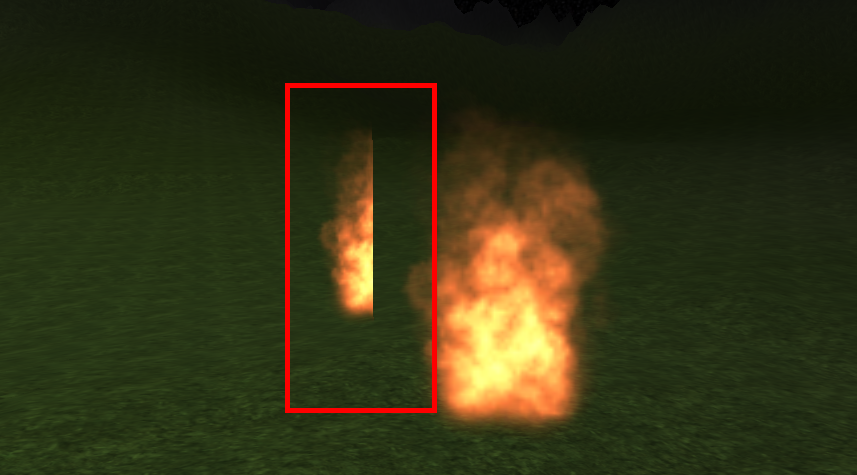
\includegraphics[width=\textwidth]{kepek/billboardOverlap.png}
 \caption{Kitakarás a blending után}
 \label{fig:spriteOverlap}
\end{figure}
\begin{figure}[h!]
 \centering
 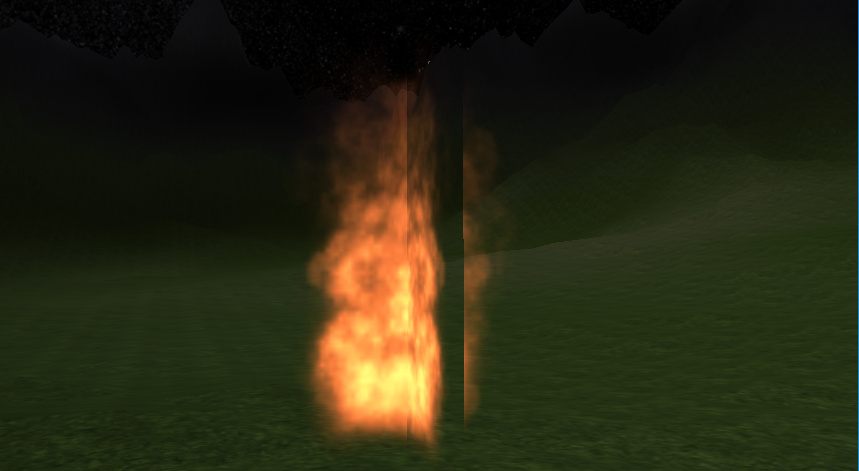
\includegraphics[width=\textwidth]{kepek/doubleBillboard1.png}
 \caption{2 síkból álló sprite probléma}
 \label{fig:doubleSprite}
\end{figure}

Így már egészen valósághű eredményt kapunk. Azonban mikor a színpuffert írjuk, gondoskodni kell róla, hogy abban már minden, a tűz hátterében feltűnő objektum színe jelen legyen.

 Ha ugyanis valamely objektum még nem került kirajzolásra a háttér elemek közül, akkor a sprite teljesen áttetsző részein sem fog szerepelni, így egy része lehet hogy átlátszósággal lesz kitakarva. Ezt figyelhetjük meg \aref{fig:spriteOverlap}. ábrán is, ahol a közelebbi sprite korábban kerül kirajzolásra, mint a mögötte lévő. A kirajzolandó objektumokat ezért a kamerától mért távolságuk alapján csökkenő sorrendben kell kirajzolni, azaz a legtávolabbiakkal kell kezdeni. Ezzel az egyszerűbb esetek meg is vannak oldva, azonban ha két objektum keresztezi egymást, mint például a 2 síkból álló billboard (\ref{fig:doubleSprite}. ábra), akkor nincs olyan kirajzolási sorrend, amely kiküszöbölné a kitakarást.

Az egyik megoldás, hogy valamelyik síkot két részre kell bontani a közepénél, így lesz 3 különböző objektum, melyeket már könnyebben sorba lehet rendezni. Hogy a \texttt{BillboardFire} osztály működését ne befolyásoljam, a \texttt{SpriteFire} osztályban a második, elforgatott sík nem az eredeti újrakirajzolásából áll majd elő, hanem egy új VAO-t hozok létre erre a célra, melyet majd két részletben rajzolok ki. Hogy ne kelljen külön forgatni, eleve az $YZ$ síkkal lesz párhuzamos. 

\begin{figure}[h]
 \centering
 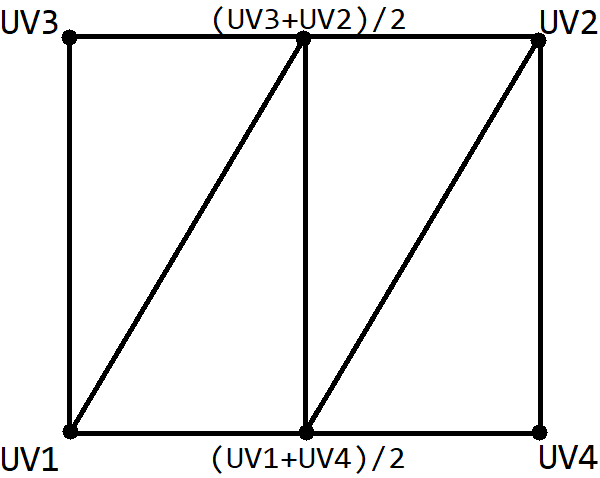
\includegraphics[width=0.5\textwidth]{kepek/billboardUVcoords.png}
 \caption{$(u, v)$ koordináták az Y tengely mentén}
 \label{fig:spriteUVcoords}
\end{figure}

A \texttt{calculateSpriteVertices} metódust kibővítettem, hogy amennyiben 2 síkot kell kirajzolni, a további 12 pontot (két külön sprite) is csatolja a visszatérési tárolóba. A pontok sorrendje itt is pontosan úgy van megadva, ahogyan az az eredeti síkon van (\ref{fig:spriteFrame}. ábra). 

A \texttt{calculateNextTextureCoordinates} metódust is hasonlóképpen egészítettem ki. Itt azonban a két sík találkozásánál található pontok textúra koordinátáit más módszerrel kellett meghatározni, mint alap esetben.
A megoldást az adott ponttal egy magasságban lévő textúra koordináták közti lineáris interpoláció jelentette, ahogyan az \aref{fig:spriteUVcoords}. ábrán is látszik. Ezt a 12 pontot szintén a vektor gyűjteményhez csatolja, mellyel visszatér.

Tehát ha kétsíkú sprite-ot kell kirajzolni, akkor a \texttt{loadVAO} metódusban a \texttt{vertices} és a \texttt{textureCoordinates} változók már 6 helyett 18 elemből állnak, melyekből két külön VAO-t kell készíteni. Az eredeti sík VAO-jában csak annyi változás történik, hogy a \texttt{glBufferData} függvény méretre vonatkozó paraméterét nem a vektor gyűjtemény méretéből számoljuk ki, hanem megadjuk, hogy 6-szor kell venni a gyűjtemény egy elemének méretét. Így csupán az első 6 elem kerül bele, ahogy az eddig is történt. A második VAO-t ehhez hasonlóan hozzuk létre, ám a \texttt{glBufferData} második (méret) és harmadik (az első elem pointere) paraméterében meg kell adni, hogy 12 elemet tároljon le a puffer 6-os indexű elemétől kezdve. Ez a csúcspontok VBO-ja esetén a következőképpen néz ki:
\begin{cpp}
glBufferData(GL_ARRAY_BUFFER, 12 * sizeof(glm::vec3), 
	&vertices[6], GL_STATIC_DRAW);
\end{cpp}

A \texttt{drawFire} metódus mellé segédmetódusoknak külön elkészítettem a \texttt{drawNormalVAO}, \texttt{drawSecondary1VAO} és \texttt{drawSecondary2VAO} metódusokat. Az első az eredeti síkot rajzolja ki, a második a (szemből nézve) bal oldali ``fél'' sprite-ot, a harmadik pedig a jobb oldalit. Ezekben csupán a VAO bindelés, valamint a \texttt{glDrawArrays} hívás található. A másodlagos (secondary) kirajzoló függvények között csupán a \texttt{glDrawArrays} hívás különbözik, az első ugyanis az első 6 elemét, a második pedig a VAO második 6 elemét rajzolja ki (\texttt{glDrawArrays(GL\_TRIANGLES, 6, 6)}). 

\begin{figure}[h]
 \centering
 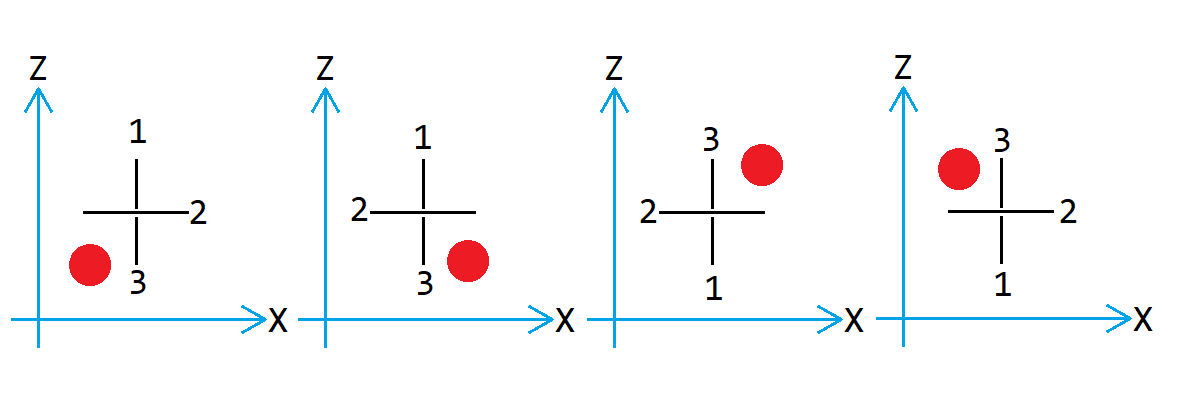
\includegraphics[width=\textwidth]{kepek/billboardSorting.png}
 \caption{Kirajzolási sorrend a ``kétsíkú'' sprite estén}
 \label{fig:spriteSorting}
\end{figure}
A kirajzoláskor a \ref{fig:spriteSorting}. ábrán látható esetek fordulhatnak elő. A piros folt a kamera helyzete, a fekete kereszt a tűz 3 külön kirajzolt sprite-ját jelképezi. A blending kedvéért a kamerától legtávolabb eső objektumokkal kell kezdeni. A renderelés sorrendjét a számok jelzik. Ez alapján jól látszik, hogy esetemben a kamera és a tűz pozíciójának $Z$ koordinátáit kell csupán összevetni, és ezek alapján két különböző kirajzolási sorrend lehetséges. 
Például az első eset (bal szélső kettő) kirajzolása: 
\begin{cpp}
if (m_pCamera->getZ() < m_vPosition.z)
{
	drawSecondary2VAO();
	drawNormalVAO();
	drawSecondary1VAO();
}
\end{cpp}
Így már kirajzoláskor minden nézőpontből helyes képet kapunk.

Ha egymás mellé kirajzolunk egy billboard és egy kétsíkú sprite objektumot, akkor \aref{fig:billboardFinal1}. ábrán látható eredményt kapjuk.

\begin{figure}[h!]
 \centering
 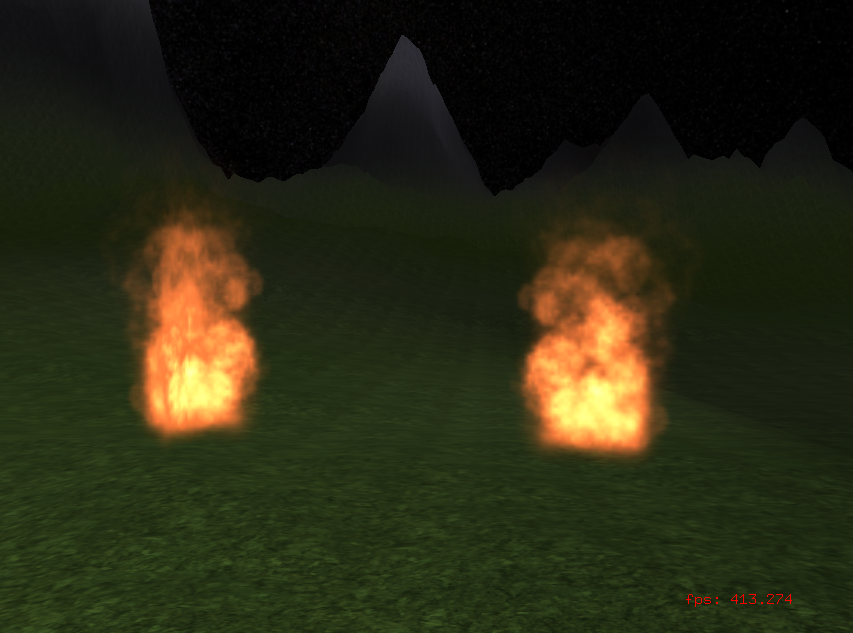
\includegraphics[width=0.95\textwidth]{kepek/billboardFinal1.png}
 \caption{Bal oldalon a kétsíkú sprite, jobb oldalon a billboard látszik.}
 \label{fig:billboardFinal1}
\end{figure}

\Aref{fig:billboardFinal2}. ábrán megfigyelhetjük, hogy a helyes sorrendbeli kirajzolásnak köszönhetően a blending szép kitakarást eredményez minden irányból.

\begin{figure}[h!]
 \centering
 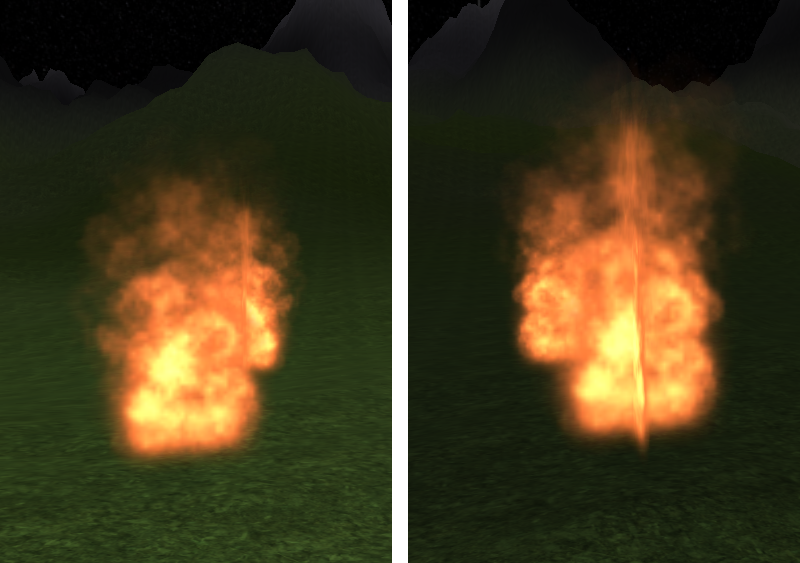
\includegraphics[width=0.85\textwidth]{kepek/billboardFinal2.png}
 \caption{Bal oldalon a billboard takar ki, jobb oldalon pedig a sprite}
 \label{fig:billboardFinal2}
\end{figure}

\Aref{fig:billboardFinal3}. ábrán mutatkozik a kétsíkú sprite egyik gyengesége. Ha ugyanazt a textúrasorozatot használjuk fel, akkor bizonyos szögekből a kép ugyanazon fele kerül egymással szembe, mely feltűnő lehet. Erre egy megoldás lehet a második síkra egy külön textúra sorozat készítése.

\begin{figure}[h!]
 \centering
 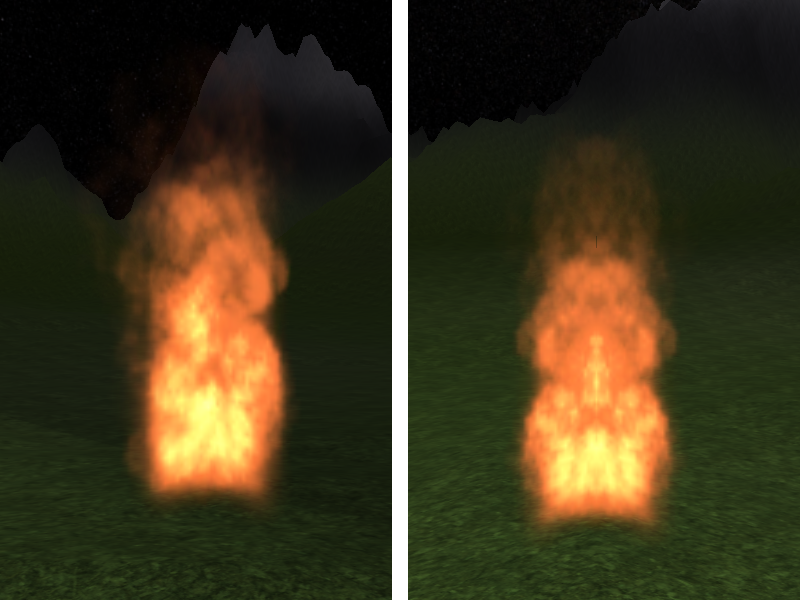
\includegraphics[width=0.85\textwidth]{kepek/billboardFinal3.png}
 \caption{A bal oldali kép esztétikusabb, a jobb oldalin feltűnő a tükröződés}
 \label{fig:billboardFinal3}
\end{figure}

\Aref{fig:billboardFinal4}. ábrán pedig megfigyelhető a kétsíkú sprite másik gyengepontja. Ha valamelyik síkra nagy szögben tekintünk, akkor feltűnővé válhat a körvonala, rombolva ezzel a látványt.

\begin{figure}[h!]
 \centering
 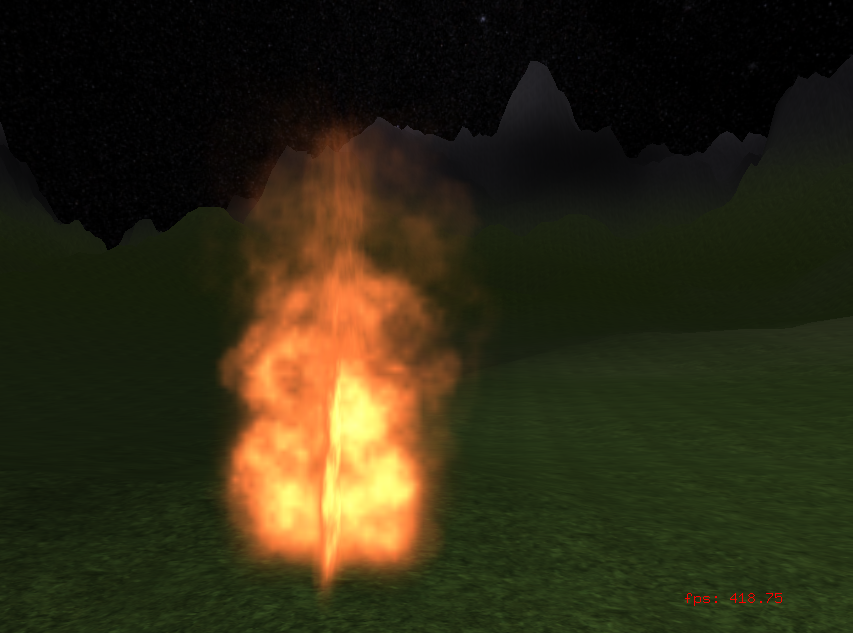
\includegraphics[width=0.85\textwidth]{kepek/billboardFinal4.png}
 \caption{Mozgás közben még szembetűnőbb a körvonal}
 \label{fig:billboardFinal4}
\end{figure}

\Aref{fig:billboardFinal5}. ábrán enyhe felülnézetből látszik igazán a két megjelenítési mód közötti különbség. Ebből a perspektívából egyik sem szerepel túl jól.

\begin{figure}[h!]
 \centering
 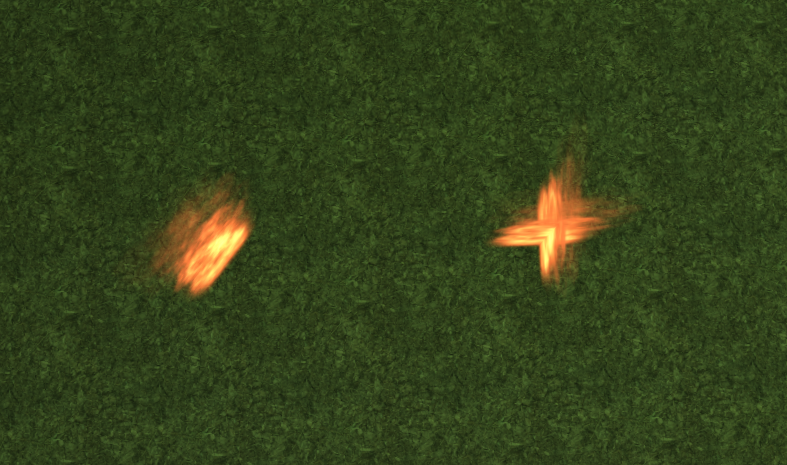
\includegraphics[width=0.85\textwidth]{kepek/billboardFinal5.png}
 \caption{Bal oldalon a billboard, jobb oldalon a sprite tűz}
 \label{fig:billboardFinal5}
\end{figure}
% Videón körbejárás, és a sebesség paraméter hatása

% fps, pontok száma, 
\subsection{Számításigény}
A másodpercenként kirajzolt képek számát egy billboard és egy 2 síkú sprite tűz nem befolyásolja, hiszen komolyabb számítást nem kell végeznie a gépnek, összesen csupán $6 \cdot 4 = 24$ pontot kell kirajzolni.


\section{Háromdimenziós részecskerendszer alapú tűz}

% FireParticle class
\subsection{FireParticle osztály}

A részecskerendszer alapú tűz részecskéinek implementálásakor a billboard alapú megjelenítést választottam váltogatható textúrával, ugyanis ezzel tudtam jelenleg a legvalószerűbb hatást elérni. Az osztályra nagyrészt egy adott részecske tulajdonságainak és helyzetének a tárolása végett volt szükség. Emellett ez végzi el képkockánként egy részecske élettartamának, pozíciójának, sebességének, méretének, elfordulásának és textúrájának a frissítését. A modell heurisztikus alapokon nyugszik, a tűz fizikai tulajdonságait utánozni próbálva. A kirajzolás nem ebben az osztályban történik.

% főbb adattagok 
\subsubsection{Adattagok}
A részecskéket a következő fontosabb tulajdonságokkal vérteztem fel:
\begin{itemize}
\item Élettartam és kor (\texttt{m\_fLifeTime}, \texttt{m\_fAge}): a kor kezdetben az élettartammal egyenlő, majd folyamatosan csökken $0$-ig.
\item Pozíció, mozgás irány, sebesség (\texttt{m\_vPosition}, \texttt{m\_vSpeedDirection}, \texttt{m\_fSpeedRate}): az irány nem egységvektor, így még nagyobb és véletlenszerűbb a különbség a részecskék mozgása között.
\item Méret és növekedési ráta (\texttt{m\_fScale}, \texttt{m\_fScaleRate}): a növekedési ráta adja meg a részecske, mint gáz tágulásának a sebességét.
\item A kamerától vett távolság (\texttt{m\_fDistanceToCamera}): ez alapján lesznek majd sorba rendezve a részecskék.
\item $Z$ tengely menti elfordulás és szögsebesség (\texttt{m\_fRotation}, \texttt{m\_fRotationRate}): ezek segítségével keltek tubulens hatást az animáció során.
\item Textúrák száma, pillanatnyi textúra sorszáma (\texttt{m\_cNumberOfTextures}, \texttt{m\_cCurrentTexture}) -- a textúrák számozása $0$-tól indul.
\item A láng és füst állapotok aránya, a pillanatnyi keverés aránya, egy jelenet ideje (\texttt{m\_fFireTimeRatio}, \texttt{m\_fCurrentBlend}, \texttt{m\_fSceneTime}): a későbbiekben kerülnek kifejtésre.
\end{itemize}

% konstruktor
\subsubsection{Konstruktor}
Az osztály konstruktora paraméterként várja az adott részecske indulási pozícióját, a sebességének irányát, az elfordulását, az élettartamát, a forgás szögsebességét, a részecske sebességét, illetve egy, a \texttt{Camera} osztály példányára mutató pointert. Ezeket lementi a megfelelő adattagokba, illetve kiszámol néhány további származtatott adatot. 

Ilyen az \texttt{m\_fSceneTime} adattag is, mely megadja, hogy a textúra sorozat egyes tagjai (melyek váltogatása a részecske animációját eredményezi) hány milliszekundumot (a továbbiakban \textit{ms}) szerepelnek. Ezt a textúrán szereplő állapotok száma és a részecske élettartamának a hányadosa adja meg. 

A füsthöz nem készítettem külön emittert és osztályt. Egy részecske az életének egy bizonyos részét lángként, utána pedig füstként tölti. A füsthöz nem alkalmaztam külön textúrát, hanem a láng képsorozat utolsó tagját használom fel kiszürkítve. Ebből következik, hogy az \texttt{m\_fSceneTime} adattagot még meg kell szorozni az \texttt{m\_fFireTimeRatio} adattaggal. Ez a $[0, 1]$ tartományon értelmezett szám adja meg, hogy a részecske az életének hanyad részét tölti láng fázisban. Ez azt is jelenti, hogy a részecske adott fázisát (láng vagy füst) az \texttt{m\_fFireTimeRatio} segítségével lehet majd meghatározni. Egy állapot tehát rövidebb ideig szerepel majd, de az utolsó jelenetet leszámítva mind ugyanannyi időt töltenek majd a képernyőn. 

% update
\subsubsection{Részecskék állapotának frissítése}
Az \texttt{update} metódus felel a részecskék karbantartásáért. A metódusnak paraméterként meg kell adni az előző frissítés óta eltelt időt ms-ban (\texttt{elapsedTime}). Ezzel első lépésként csökkentjük a részecske kprát, majd megvizsgáljuk, hogy életben van-e még ($\texttt{m\_fAge} > 0$). Ha nem, akkor a függvény hamis értékkel tér vissza, ha igen, akkor frissíti az adattagokat, majd igaz értéket ad vissza. A frissítéshez két segédváltozó szükséges: a lépték és a részecske relatív kora (\texttt{step}, \texttt{relativeAge}). A léptéket az eltelt idő század részének választottam meg, a relatív kor pedig a részecske korának és élettartamának hányadosa, azaz 1-től indul és végül 0-hoz ér el. Az adattagokat a következők alapján módosítottam: 
\begin{cpp}
// Slowing x and z much faster than y
m_vSpeedDirection.x /= 1.f + step * 0.05f * relativeAge;
m_vSpeedDirection.z /= 1.f + step * 0.05f * relativeAge;
m_fSpeedRate /= 1.f + step * 0.01 * (1-relativeAge);

// Extra forces
if (m_bForceApplied)
{
	m_vPosition += m_vForceDirection * m_fForceSpeed * step;
	m_bForceApplied = false;
}

// Moving
m_vPosition += m_vSpeedDirection * step * m_fSpeedRate;

// Expanding
m_fScale += m_fScaleRate * step;

// Rotate
m_fRotation += step * m_fRotationRate;

// Changing texture
{...}

m_fDistanceToCamera = glm::distance2(
		m_vPosition, m_pCamera->getPosition());
\end{cpp}
A lépték változóval történő szorzás a korábbiakban tárgyalt okokból kifolyóan történik, hogy az adattagok az eltelt idő függvényében változzanak. A relatív életkorral történő szorzás pedig olyan esetekben volt szükséges, mikor a változást a részecske korától is függővé kellett tenni.

A sebesség irányának $x$ és $z$ koordinátáit azért kellett nagyobb mértékben csökkenteni, hogy a részecskék ne egyenes vonalban távolodjanak egymástól, mint például egy robbanás esetén, hanem parabolaszerűen egyre függőlegesebben emelkedjenek (\ref{fig:parabolicSpeedVector}. ábra). A részecske korának csökkenésével (azaz az öregedésével) egyre kisebb mértékű a csillapítás is.
\begin{figure}[h]
 \centering
 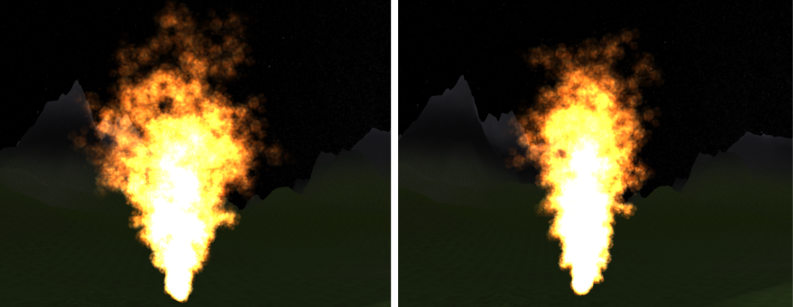
\includegraphics[width=\textwidth]{kepek/parabolicSpeedVector.png}
 \caption{Bal oldalon a csillapítás nélküli, jobb oldalon a lassított $x$ és $z$ koordinátákkal kapott eredmény.}
 \label{fig:parabolicSpeedVector}
\end{figure}
A részecskék sebességét viszont annál jobban csökkentettem, minél közelebb ér élete végéhez. 

A külső erőket egy publikus metódus (\texttt{applyForce(glm::vec3 direction, float speed)}) segítségével lehet hozzáadni, ám ezt minden frissítés előtt meg kell tenni. Ez azért alakult így, mert a külső erőket más osztályok szabályozzák, de képkockáról képkockára változhatnak azok is. A megadott irányba a megadott sebességgel hatok a részecske pozíciójára a frissítés során.

A kamerától vett távolság kiszámításakor a négyzetes távolságot veszem (\texttt{glm::distance2}), így egy gyökvonást megspórolok, de a végső sorrenden ez úgysem változtat. A mozgatás, tágulás és forgatás nem igényelnek különösebb magyarázatot.

%textúrázás
\subsubsection{Textúrázás}
A textúrázás a billboard alapú tűznél alkalmazott módszerre hasonlít. Mivel a textúra koordinátákat részecskénként ki kell számolni, és egyszerre két jelenet koordinátáira is szükség van, részecskénként $6 \cdot 4 = 24$ db \texttt{float} koordinátát kellene átküldeni (és a lassú CPU-n kiszámolni) az árnyalónak. Mivel egyébként is sok információt kell nekik eljuttatni, és az adatmozgatás a shaderek felé aránylag lassú művelet, inkább a vertex shader-ben végzem a koordináták meghatározását. Ahhoz, hogy ott el tudjam végezni a műveletet szükség van azonban a pillanatnyi textúra sorszámára. Ennek meghatározáa során oda kell figyelni arra is, hogy a részecske láng, vagy füst fázisban van-e.

\begin{cpp}
// Changing texture
float textureInfo = (m_fLifeTime - m_fAge) / m_fSceneTime;
m_cCurrentTexture = (int)textureInfo;
if (m_cCurrentTexture < m_cNumberOfTextures)
{
	// Flame
	m_fCurrentBlend = 1.f - fmod(textureInfo, 1.0f);
}
else
{
	// Smoke
	m_cCurrentTexture = m_cNumberOfTextures;
	// fade the somke out
	m_fCurrentBlend = relativeAge / (1 - m_fFireTimeRatio);
	m_fScale += 0.1 *step;
}
\end{cpp}

A \texttt{textureInfo} segédváltozóban kiszámolom, hogy a születés óta eltelt idő alatt hányszor telt el az egy jelenetre jutó idő. Ennek az egész része adja meg a pillanatnyi textúra sorszámát (\texttt{m\_cCurrentTexture}). Ha ez a szám nem kisebb, mint a textúrák száma, az azt jelenti hogy a részecske már a füst fázisban tart.

Hogy az animáció még folyékonyabb legyen a láng fázisban, egyszerre két jelenetet használok fel a textúrán található képsorozatból: a pillanatnyi textúrát, és az utána következőt. Ezt a kettőt mosom össze annak alapján, hogy a pillanatnyi textúrára jutó időből mennyi van még hátra. Az ehhez szükséges arányszámot tárolom az \texttt{m\_fCurrentBlend} adattagban. Tehát először csak a pillanatnyi textúra látszik ($\texttt{m\_fCurrentBlend} = 1$), majd ahogy telik az idő, a pillanatnyi textúra egyre jobban halványodik, a következő pedig erősödik. Ebből kifolyólag az \texttt{m\_cNumberOfTextures} adattagban valójában a textúrák számától eggyel kisebb számot tárolok, különben az utolsó jelenetet nem lenne mivel összemosni.

Füst fázisban a \texttt{m\_fCurrentBlend} adattag már nem összemosásra, hanem elhalványításra használatos. Az $1 - \texttt{m\_fFireTimeRatio}$ adja meg a füstként töltendő időt ($[0, 1]$ tartományban). Mikor a program ehhez a részhez ér, biztos, hogy a relatív kor is maximum ennyi lehet, így a kettő hányadosa megmutatja, hogy mennyi van még hátra a füst fázisból (szintén $[0, 1]$ tartományban). Tehát mire a fázis (és egyben élete) végéhez ér a részecske, teljesen elhalványodik. Füst fázisban a tágulás is nagyobb mértékű, mert az elhalványodással együtt így olyan hatást kelt, mintha a füst eloszlana a levegőben.

\begin{figure}[h]
 \centering
 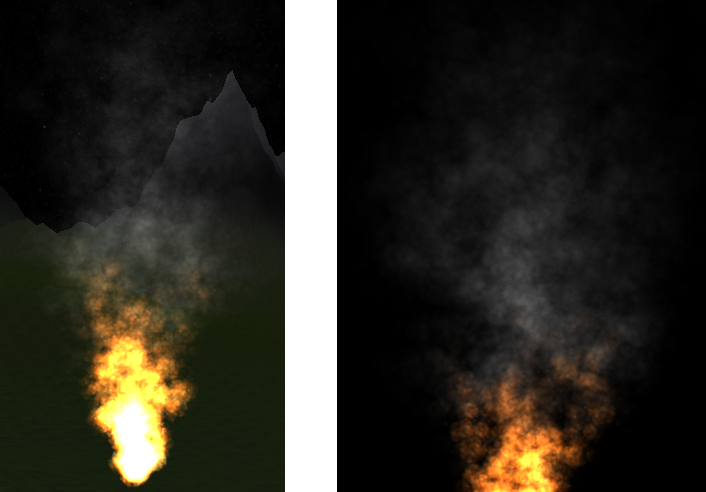
\includegraphics[width=\textwidth]{kepek/particleFireSmoke.png}
 \caption{Bal oldalon a tűz $\texttt{m\_fFireTimeRatio} = 0.25$ paraméterrel, jobb oldalon pedig a füst eloszlása közelebbről}
 \label{fig:particleFireSmoke}
\end{figure}

\subsubsection{Egyéb metódusok}
A részecskék rendezésére a későbbiekben az \texttt{std::sort} függvény segítségével kerül sor. Ennek azonban szüksége van az összehasonlításhoz valamilyen függvényre, vagy a $<$ operátor felüldefiniálására. Én az utóbbi megoldást választottam: 
\begin{cpp}
inline bool FireParticle::operator<(const FireParticle & rhs)
{
	return m_fDistanceToCamera > rhs.getDistanceToCamera();
}
\end{cpp}
Az \texttt{std::sort} ezt az operátort felhasználva növekvő sorrendbe teszi az objektumokat egy adott tárolón belül. Mivel a kamerától távolabbi részecskéket szeretném előbb kirajzolni, két részecske közül a nagyobb távolsággal rendelkezőt definiáltam kisebbnek.

A \texttt{FireParticle} osztály rendelkezik még jó néhány ``getter'' metódussal, melyek az árnyalóknak küldendő információkat adják vissza egyesével.

% FireParticleSystem



% additive(no sort, less particles) vs traditional blending

% Depth-et kikapcsolni, mert a közeli particle-ök sorba rendezve is kitakarják egymást
%Erre az egyik megoldás lehet a mélység puffer (depth buffer) írásának kikapcsolása a rajzolás idejére. A mélység puffer a színpufferhez hasonlóan pixelenként tárolja az információt. A feladata, hogy a nézőponthoz közelebbi objektumokat ne takarják ki az attól távolabbiak. Ha engedélyezve van a használata, akkor a fragment shader kimeneti értékének a mélységét összeveti a pufferben az annak megfelelő helyen tárolt értékkel. Ha az új kimenet értéke nagyobb, azaz távolabb van a kamerától, akkor nem íródik be az érték sem a mélység, sem a szín pufferbe. Ezt a funkcionalitást a glDepthMask(GL_FALSE) függvény segítségével lehet felfüggeszteni. Ekkor a színeket bármiféle vizsgálat nélkül írja a szín pufferbe.












